%-------------------------------------------------------------------------------
%-------------------------------------------------------------------------------
%-------------------------------------------------------------------------------
\chapter{Méthode de Monte-Carlo}
%-------------------------------------------------------------------------------
%-------------------------------------------------------------------------------
\thispagestyle{empty}
%-------------------------------------------------------------------------------
\vskip -1cm
{\sf Ce T.P. a pour but 
\begin{itemize}
    \item de définir la distribution d'un grand nombre de données et la présentation associée,  un histogramme,
    \item d'utiliser la méthode de Monte-Carlo pour illustrer la transmission des incertitudes lors de calculs.
\end{itemize}
}
%-------------------------------------------------------------------------------
%-------------------------------------------------------------------------------
%-------------------------------------------------------------------------------
\section{Histogrammes}
%-------------------------------------------------------------------------------
%-------------------------------------------------------------------------------
%-------------------------------------------------------------------------------
{\it En statistique, un histogramme est une représentation graphique permettant de représenter la répartition d'une variable continue en la représentant avec des colonnes verticales. } (Wikipedia)

Nous partons d'une liste de valeurs qui représentent les variations d'une mesure :
\begin{itemize}
    \item les diamètres de pièces usinées,
    \item les tailles des enfants de 4 ans,
    \item les luminosités des pixels d'une photographie,
    \item les différentes mesures d'un pH lors d'un T.P. \dots
\end{itemize}
%-------------------------------------------------------------------------------
%-------------------------------------------------------------------------------
\subsection{Premières mesures}
%-------------------------------------------------------------------------------
%-------------------------------------------------------------------------------
La première approche est de calculer
\begin{enumerate}
    \item la moyenne pour obtenir une valeur centrale, 
    \item l'écart-type (racine de la variance) pour obtenir un ordre de grandeur de la dispersion autour de la moyenne
    \item le maximum et le minimum pour obtenir un encadrement des valeurs.
\end{enumerate}
%--------------------------------------------------------------------------
%--------------------------------------------------------------------------
\begin{Exercise}\it Écrire une fonction \type{moyenne(liste)} qui calcule la moyenne d'une liste.
\end{Exercise}
%--------------------------------------------------------------------------
%--------------------------------------------------------------------------
\begin{Answer}
\begin{lstlisting}
def moyenne(liste):
    n = len(liste)
    s = 0
    for x in liste:
        s = s + x
    return s/n
\end{lstlisting}
\end{Answer}
%--------------------------------------------------------------------------
%--------------------------------------------------------------------------
\begin{Exercise}\it Écrire une fonction \type{ecart\_type(liste)} qui calcule l'écart-type d'une liste.

Rappel : la variance d'une liste est la moyenne des $(x_i-m)^2$ où $m$ est la moyenne des $x_i$ c'est aussi la moyenne des carrés, $x_i^2$, à laquelle on soustrait $m^2$.
\end{Exercise}
%--------------------------------------------------------------------------
%--------------------------------------------------------------------------
\begin{Answer}
\begin{lstlisting}
def ecart_type(liste):
    n = len(liste)
    m = moyenne(liste)
    s = 0
    for x in liste:
        s = s + (x-m)**2
    return (s/n)**0.5
\end{lstlisting}
\end{Answer}
%--------------------------------------------------------------------------
%--------------------------------------------------------------------------
\begin{Exercise}\it Écrire une fonction \type{maximum(liste)}, resp. \type{minimum(liste)},  qui calcule le maximum, resp.le minimum, des termes d'une liste. On pourra supposer que la liste est non vide.
\end{Exercise}
%--------------------------------------------------------------------------
%--------------------------------------------------------------------------
\begin{Answer}
\begin{lstlisting}
def maximum(liste):
    maxi = liste[0]
    for x in liste:
        if x > maxi:
            maxi = x
    return maxi
\end{lstlisting}

\begin{lstlisting}
def minimum(liste):
    mini = liste[0]
    for x in liste:
        if x < mini:
            mini = x
    return mini
\end{lstlisting}
\end{Answer}
%-------------------------------------------------------------------------------
%-------------------------------------------------------------------------------
\subsection{Comptage}
%-------------------------------------------------------------------------------
%-------------------------------------------------------------------------------
On peut aller plus loin en découpant un intervalle contenant les valeurs en plusieurs sous-intervalles (on parle de {\bf bins}) et comptant le nombre de valeurs de la liste dans chacun de ces intervalles.

On choisit la méthode suivante :
\begin{enumerate}
    \item on choisit le nombre d'intervalles, $n$
    \item on calcule le minimum, \type{mini}, et le maximum, \type{maxi}, des valeurs de la liste
    \item on détermine les intervalles, $I_0 = [a_0; a_1[,\ I_1 = [a_1; a_2[,\ \cdots I_{n-1} = [a_{n-1};a_n]$
    
    avec $a_k = \type{mini} + k.h$ et $h = \frac 1n\bigl(\type{maxi}-\type{mini}\bigr)$,
    \item on crée une liste de taille $n$ initialisée à 0, \type{histo},
    \item pour chaque valeur $x$, on détermine l'intervalle auquel $x$ appartient, $I_k$, et on incrémente la valeur de \type{histo[k]} de 1.
\end{enumerate}

On remarque que $x$ appartient à $I_k$ si et seulement si $a_k\le x < a_{k+1}$, c'est-à-dire 
$k.h \le x - \type{mini} < (k+1).h$ d'où $\displaystyle k =\left\lfloor\frac{x - \type{mini}}h\right\rfloor$.
Il y a cependant un cas particulier : si $x=\type{maxi}$ alors $\displaystyle \left\lfloor\frac{x - \type{mini}}h\right\rfloor$ vaut $n$ mais il faut compter $x$ dans $I_{n-1}$.

%--------------------------------------------------------------------------
%--------------------------------------------------------------------------
\begin{Exercise}\it Écrire une fonction \type{comptage(liste, n)} qui renvoie le nombre d'éléments par intervalle dans une liste \type{histo} selon l'algorithme ci-dessus ainsi que le pas $h$ et la valeur du minimum.
\end{Exercise}
%--------------------------------------------------------------------------
%--------------------------------------------------------------------------
\begin{Answer}
\begin{lstlisting}
def comptage(liste, n):
    mini = minimum(liste)
    maxi = maximum(liste)
    h = (maxi - mini)/n
    histo = [0]*n
    for x  in liste:
        k = int((x-mini)/h)
        if k == n:
            k = n - 1
        histo[k] += 1
    return histo, h, mini
\end{lstlisting}
\newpage
\end{Answer}
%--------------------------------------------------------------------------
%--------------------------------------------------------------------------
Dans le cas \type{L0 = [4.3, 5.1, 7.8, 5.4, 4.4, 7.3, 6.8, 6.7, 5.9, 7.1]}, 

\type{comptage(L0, 5)} renvoie \type{([2, 2, 1, 2, 3], 0.7, 4.3)}.

{\sf Un fonction semblable existe dans le module \type{numpy} : \type{np.histogram}}
%-------------------------------------------------------------------------------
%-------------------------------------------------------------------------------
\subsection{Affichage}
%-------------------------------------------------------------------------------
%-------------------------------------------------------------------------------
Pour obtenir la représentation graphique des valeurs calculées, on utilise un diagramme en barres disponible avec la fonction \type{plt.bar} où \type{plt} est le nom donné au module graphique de Python.
\begin{lstlisting}
import matplotlib.pyplot as plt
\end{lstlisting}
Cette fonction a deux paramètres obligatoires et de nombreux paramètres optionnels (nommés) dont nous n'allons utiliser qu'un seul : \type{width}.

\type{plt.bar(X, Y, width = w)} reçoit 3 paramètres 
\begin{enumerate}
    \item \type{X} est la liste des centres des intervalles $I_k$ définis ci-dessus,
    \item \type{Y} est la liste, de même longueur que \type{X}, des nombres d'éléments dans chaque intervalle,
    \item \type{w} est la largeur.
\end{enumerate}
Si $n$ est la longueur des listes \type{X} et \type{Y}, la fonction va tracer $n$ rectangles pour $0\le i < n$, dont la base est le segment $\bigl[X[i] - w/2; X[i] + w/2\bigr]$ sur l'axe des abscisses et dont
la hauteur est $Y[i]$.

Les points $X[i]$ ne sont pas obligatoirement régulièrement espacés et les $Y[i]$ peuvent être des réels.

Par exemple \type{plt.bar([1, 2, 3, 5], [3, 5, 4, 2.5], width = 0.8)} donne
%-------------------------------------------------------------------------------
\begin{center}
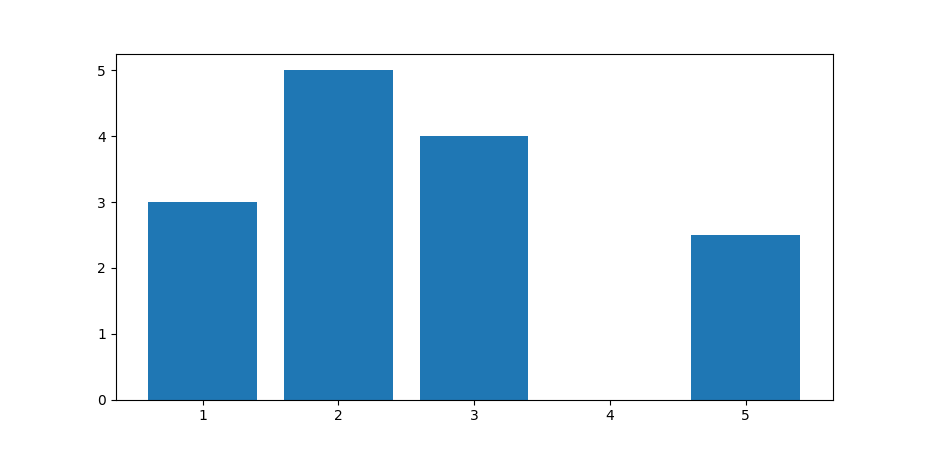
\includegraphics[scale=0.4]{TP/Images/TP17_histo1.png}
\end{center}
%-------------------------------------------------------------------------------

\newpage
On peut donc écrire la fonction
%--------------------------------------------------------------------------
\begin{lstlisting}
def histogramme(liste, n):
    valeurs, h, mini = comptage(liste, n)
    centres = ....
    for i in range(n):
        ....
    plt.bar(centres, valeurs, width = h)
    plt.show()
\end{lstlisting}
%--------------------------------------------------------------------------
\type{histogramme(L0, 5)} donne le résultat suivant.
%-------------------------------------------------------------------------------
\begin{center}
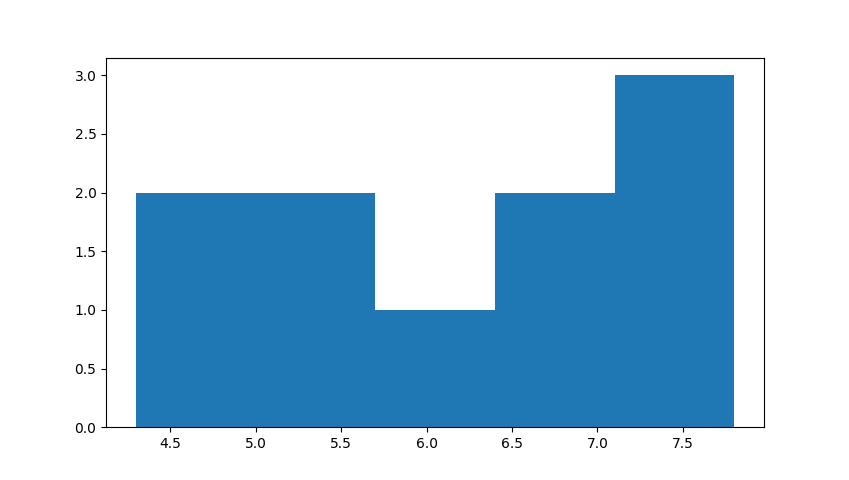
\includegraphics[scale=0.4]{TP/Images/TP17_histo2.png}
\end{center}
%--------------------------------------------------------------------------
%--------------------------------------------------------------------------
\begin{Exercise}\it 
Compléter le code ci-dessus pour calculer la liste des centres.
\end{Exercise}
%--------------------------------------------------------------------------
%--------------------------------------------------------------------------
\begin{Answer}
\begin{lstlisting}
def histogramme(liste, n):
    valeurs, h, mini = comptage(liste, n)
    centres = [0]*n
    for i in range(n):
        centres[i] = mini + (i+1/2)*h
    plt.bar(centres, valeurs, width = h)
    plt.show()
\end{lstlisting}
\end{Answer}
%-------------------------------------------------------------------------------
%-------------------------------------------------------------------------------
Cette fonction est semblable à la fonction \type{plt.hist(liste, bins = n)}
%-------------------------------------------------------------------------------
%-------------------------------------------------------------------------------
%-------------------------------------------------------------------------------
\section{Simulation des incertitudes}
%-------------------------------------------------------------------------------
%-------------------------------------------------------------------------------
%-------------------------------------------------------------------------------
Nous allons utiliser la représentation par histogrammes pour illustrer la propagation des incertitudes simples.
%-------------------------------------------------------------------------------
%-------------------------------------------------------------------------------
\subsection{Incertitude d'une valeur}
%-------------------------------------------------------------------------------
%-------------------------------------------------------------------------------
On considère, par exemple, un volume de 12,5 ml mesuré à la pipette graduée ; on sait le volume réel est compris entre 12,45 ml et 12,55 ml, l'incertitude dépend entre autres de la dextérité du manipulateur.

On va simuler cette incertitude en produisant une liste de valeurs aléatoirement choisies dans l'intervalle. Pour cela on utilisera la fonction \type{rd.random} du module \type{random}
%--------------------------------------------------------------------------
\begin{lstlisting}
import random as rd
\end{lstlisting}
%--------------------------------------------------------------------------
\type{rd.random()} renvoie un flottant choisi aléatoirement dans l'intervalle $[0;1[$.
%--------------------------------------------------------------------------
%--------------------------------------------------------------------------
\begin{Exercise}\it 
Écrire une fonction \type{liste\_alea(x0, e, n)} qui renvoie une liste de taille $n$ dont les valeurs sont choisies aléatoirement dans l'intervalle $[x_0 - e; x_0 + e]$.
\end{Exercise}
%--------------------------------------------------------------------------
%--------------------------------------------------------------------------
\begin{Answer}
\begin{lstlisting}
def liste_alea(x0, e, n):
    out = [0]*n
    for i in range(n):
        x = x0 + (2*rd.random() - 1)*e
        out[i] = x
    return out
\end{lstlisting}
\end{Answer}
%--------------------------------------------------------------------------
%--------------------------------------------------------------------------
\begin{minipage}{0.6\linewidth}
Si on représente l'histogramme de la liste \type{liste\_alea(12.5, 0.05, 10000)} avec 20 intervalles, on obtient des valeurs presque égales.
\end{minipage}
\begin{minipage}{0.4\linewidth}
\begin{center}
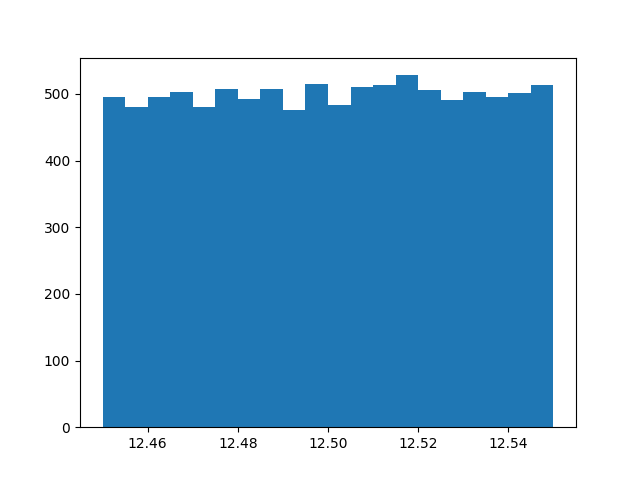
\includegraphics[scale=0.3]{TP/Images/TP17_histo3.png}
\end{center}
\end{minipage}
%-------------------------------------------------------------------------------
%-------------------------------------------------------------------------------
\subsection{Opérations}
%-------------------------------------------------------------------------------
%--------------------------------------------------------------------------
\begin{Exercise}\it 
On se donne deux simulations \type{A = liste\_alea(12.5, 0.05, 10000)} et 

\type{B = liste\_alea(8.3, 0.05, 10000)}. Déterminer la liste \type{X} telle que \type{X[i] = A[i] + B[i]} et représenter son histogramme avec 20 intervalles.
\end{Exercise}
%--------------------------------------------------------------------------
%--------------------------------------------------------------------------
\begin{Answer}
\begin{lstlisting}
A = liste_alea(12.5, 0.05, 10000)
B = liste_alea(8.3, 0.05, 10000)
X = [A[i] + B[i] for i in range(len(A))]
histogramme(X, 20)
\end{lstlisting}
\end{Answer}
%--------------------------------------------------------------------------
%--------------------------------------------------------------------------
\begin{Exercise}\it 
On se donne deux simulations \type{A = liste\_alea(12.5, 0.05, 10000)} et 

\type{B = liste\_alea(8.32, 0.005, 10000)}. Déterminer la liste \type{X} telle que \type{X[i] = A[i] + B[i]} et représenter son histogramme avec 20 intervalles.

Comparer avec le cas précédent, commentez.
\end{Exercise}
%--------------------------------------------------------------------------
%--------------------------------------------------------------------------
\begin{Answer}
\begin{lstlisting}
A = liste_alea(12.5, 0.05, 10000)
B = liste_alea(8.32, 0.005, 10000)
X = [A[i] + B[i] for i in range(len(A))]
histogramme(X, 20)
\end{lstlisting}
Les 2 incertitudes ne se combinent pas pour former une distribution triangulaire car l'une est petite devant l'autre. On peut considérer qu'il n'y a que l'incertitude sur $A$.
\end{Answer}
%--------------------------------------------------------------------------
%--------------------------------------------------------------------------
\begin{Exercise}\it  Calculer des simulations sur 10000 points de valeurs $a= 12,5$, $b = 8,3$, $c = 4,7$ et $d = 13,4$, chacune avec une précision $\pm 0,05$.

Calculer et représenter les valeurs de $\displaystyle x = \frac{a+b}{c+d}$.
\end{Exercise}
%--------------------------------------------------------------------------
%--------------------------------------------------------------------------
\begin{Answer}
\begin{lstlisting}
A = liste_alea(12.5, 0.05, 10000)
B = liste_alea(8.3, 0.05, 10000)
C = liste_alea(4.7, 0.05, 10000)
D = liste_alea(13.4, 0.05, 10000)
X = [(A[i] + B[i])/(C[i]+D[i]) for i in range(len(A))]
histogramme(X, 20)
\end{lstlisting}
On obtient une distribution qui ressemble à une gaussienne.
\begin{center}
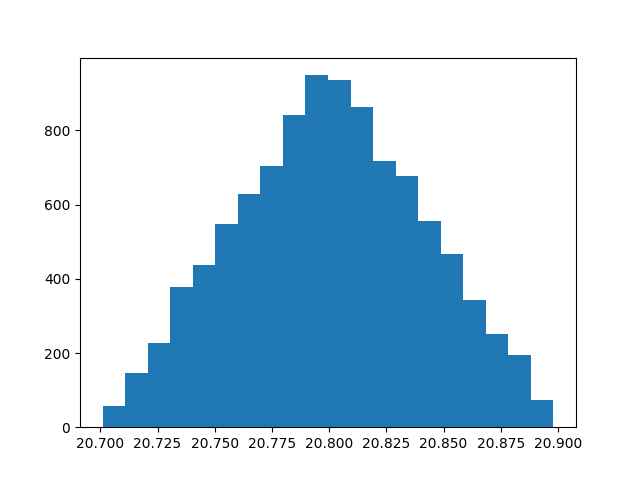
\includegraphics[scale=0.3]{TP/Images/TP17_histo4.png}
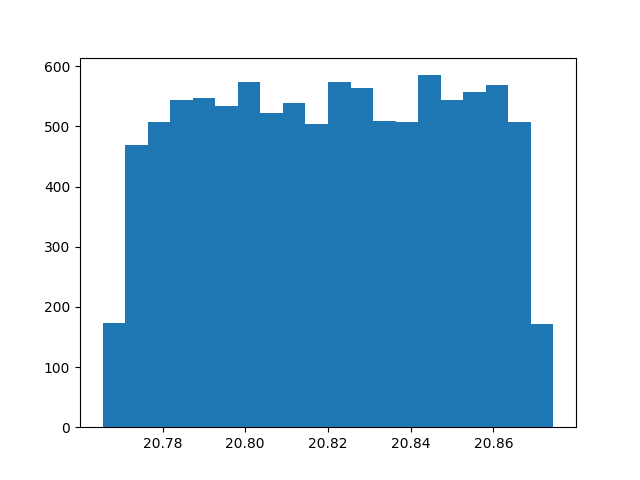
\includegraphics[scale=0.3]{TP/Images/TP17_histo5.png}
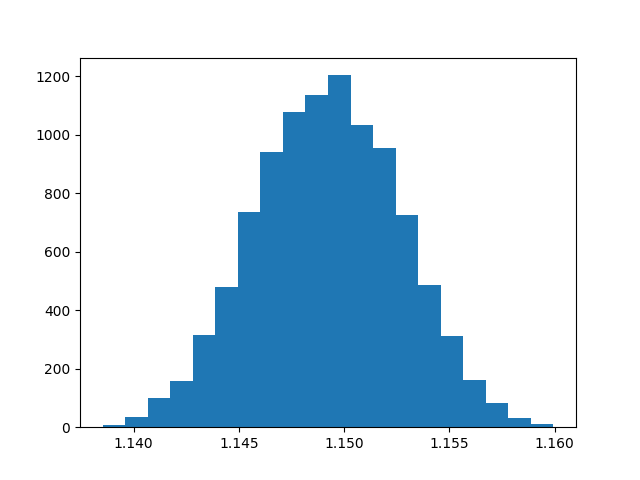
\includegraphics[scale=0.3]{TP/Images/TP17_histo6.png}
\end{center}
\newpage
\end{Answer}
%-------------------------------------------------------------------------------
%-------------------------------------------------------------------------------
\subsection{Vers une gaussienne}
%-------------------------------------------------------------------------------
%--------------------------------------------------------------------------
Un comportement souvent observé est que si on combine plusieurs incertitudes on s'approche d'une gaussienne.
%--------------------------------------------------------------------------
%--------------------------------------------------------------------------
\begin{Exercise}\it 
\begin{enumerate}
    \item Créer une liste de taille 100 dont les éléments sont des simulations sur 100000 points d'une valeur $a= 12,5$ avec une précision $\pm 0,05$. On obtient une liste de listes de taille $100\times 100\,000$.
    \item Calculer et représenter les valeurs de la liste \type{M} de taille $100\,000$ telle que \type{M[i]} est la moyenne des \type{X[k][i]} pour $k$ variant de 0 à 99.
    \item Calculer la moyenne $m$ et l'écart-type $\sigma$ de \type{M}.
\end{enumerate}
\end{Exercise}
%--------------------------------------------------------------------------
%--------------------------------------------------------------------------
\begin{Answer}
\begin{lstlisting}
import math
N = 100000
N1 = 100
A = [0]*N1
for i in range(N1):
    A[i] = liste_alea(12.5, 0.05, N)

M = [0]*N
for i in range(N):
    s = 0
    for k in range(N1):
        s = s + A[k][i]
    M[k] = s/N1

def gauss(x, m, s):
    return math.exp(-(x-m)**2/2/s**2)/s/(2*math.pi)**0.5

def histogramme_gauss(liste, n):
    valeurs, h, mini = comptage(liste, n)
    centres = [0]*n
    for i in range(n):
        centres[i] = mini + (i+1/2)*h
    plt.bar(centres, valeurs, width = h)
    m = moyenne(M)
    s = ecart_type(M)
    X = [m - 4*s + i*8*s/1000 for i in range(1000)]
    Y = [N*h*gauss(x, m, s) for x in X]
    plt.plot(X, Y, color="red")
    plt.show()


histogramme_gauss(M, 50)
\end{lstlisting}
\end{Answer}
%-------------------------------------------------------------------------------
%-------------------------------------------------------------------------------


On pourra comparer avec une gaussienne sur le même graphe.

La fonction est de la forme $\displaystyle x \mapsto \frac{K}{\sqrt{2\pi}\sigma}\exp\left(\frac{-(x-m)^2}{2\sigma^2}\right)$ 
où $K$ est la surface de l'histogramme : c'est le nombre de points multiplié par $h$, la largeur des intervalles.
%-------------------------------------------------------------------------------
\begin{center}
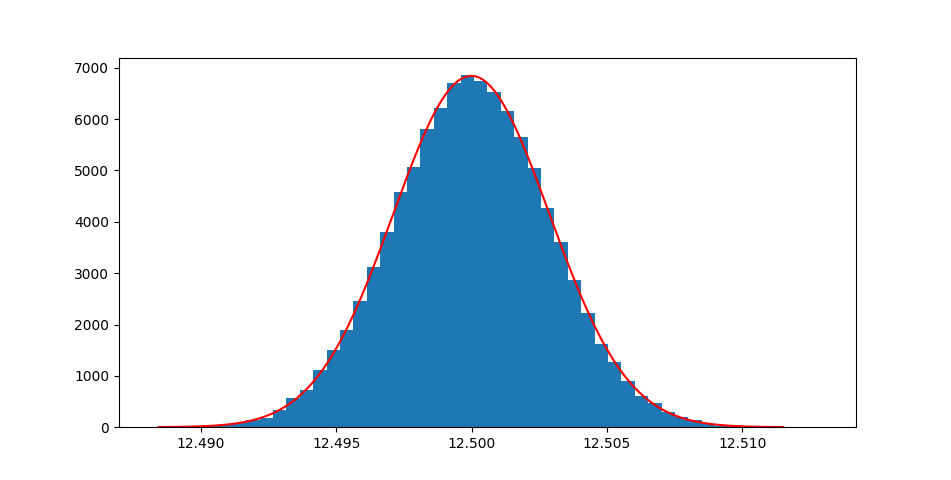
\includegraphics[scale=0.6]{TP/Images/TP17_histo7.png}
\end{center}
%--------------------------------------------------------------------------


